\documentclass{beamer}

%--------------beamer---------------
\usetheme{Warsaw}
\usecolortheme{rose}
\usefonttheme{professionalfonts}
\usepackage{tikz}
\useinnertheme{rectangles}
\useoutertheme{miniframes}
\setbeamercolor*{mini frame}{fg=black,bg=white}
\definecolor{blizzardblue}{rgb}{0.67, 0.9, 0.93}
\setbeamercolor{section in head/foot}{fg=black, bg=blizzardblue}

\defbeamertemplate{subsection in toc}{bullets}{%
  \leavevmode
  \parbox[t]{1em}{\textbullet\hfill}%
  \parbox[t]{\dimexpr\textwidth-1em\relax}{\inserttocsubsection}\par}
\defbeamertemplate{section in toc}{sections numbered roman}{%
  \leavevmode%
  \MakeUppercase{\romannumeral\inserttocsectionnumber}.\ %
  \inserttocsection\par}

\setbeamertemplate{section in toc}[sections numbered roman]
\setbeamertemplate{subsection in toc}[bullets]


%-------------packages--------------
\usepackage{graphicx} 
\usepackage{hyperref}
\setbeamertemplate{caption}{\raggedright\insertcaption\par}
	
\usetikzlibrary{shapes.geometric}

%------------title page-------------

\addtobeamertemplate{navigation symbols}{}{%
    \usebeamerfont{footline}%
    \usebeamercolor[fg]{footline}%
    \hspace{1em}%
    \insertframenumber/\inserttotalframenumber
}
\title{Maximum Bipartite Matching}
\author[Jahin $(2005012)$, Amim $(2005017)$ \& Tazwar $(2005020)$]
{Abrar Jahin Sarker\inst{1} \newline Abdullah  Muhammed  Amimul Ehsan\inst{2} \newline Mostafa Rifat Tazwar\inst{3}}
\institute[VFU] % (optional)
{
  \inst{1}$2005012$
  \and
  \inst{2}$2005017$
  \and
  \inst{3}$2005020$
  \and
  \inst{1,2,3}Department of Computer Science and Technology, BUET
}
\date{February 11, 2024}

\AtBeginSection
{
\begin{frame}{Outline}
    \tableofcontents[currentsection]
\end{frame}
}

\begin{document}

\begin{frame}
    \titlepage
\end{frame}

\begin{frame}{Table Of Contents}
    \tableofcontents
\end{frame}

% insert introduction

\section{Introduction}
\begin{frame}{Introduction}
    

\begin{block}{Definition}
    A bipartrite graph is one whose vertices can be split into two independent groups U,V such that every edge connects between U and V.
\end{block}
\begin{alertblock}{Note}
 There can not be any edge in between U and in between V .\\
     The graph is two colourable and doesn't have  cycles of odd length.

\end{alertblock}

    \begin{figure}
        \centering
        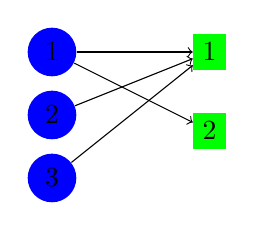
\begin{tikzpicture}
            % Boys
            \node[fill=blue, circle] (b1) at (0,0) {1};
            \node[fill=blue, circle] (b2) at (0,-0.8) {2};
            \node[fill=blue, circle] (b3) at (0,-1.6) {3};
            
            % Girls
            \node[fill=green, rectangle] (g1) at (2,0) {1};
            \node[fill=green, rectangle] (g2) at (2,-1) {2};
            
            % Potential Pairs
            \draw[->] (b1) -- (g1);
            \draw[->] (b1) -- (g2);
            \draw[->] (b2) -- (g1);
            \draw[->] (b3) -- (g1);
            

        \end{tikzpicture}
        \caption{Fig: Visualization of bipartrite graph}
    \end{figure}

\end{frame}
    


\section{The Problem}

\begin{frame}{The Problem}
\begin{block}{Maximum Bipartite Matching}
     Given a bipartite graph $G = (A \cup B, E)$, find an \\ \{ $S \subseteq A \times B$ : $S$ is a matching and is as large as possible. \} \cite{kleinberg2006algorithm}
    \end{block}
\end{frame}

\section{Example}

\begin{frame}{Example}
In a picnic,there are 5 people and 5 food items.Some people express interest in some of the items.How can we satisfy maximum number of people while wasting minimum number of items?

        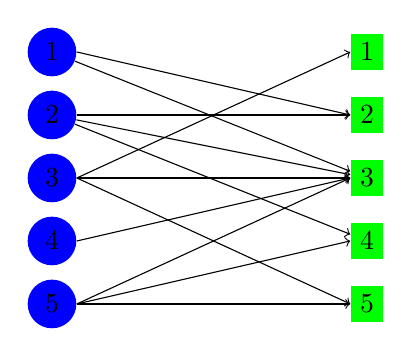
\begin{tikzpicture}
            % Boys
            \node[fill=blue, circle] (p1) at (0,0) {1};
            \node[fill=blue, circle] (p2) at (0,-0.8) {2};
            \node[fill=blue, circle] (p3) at (0,-1.6) {3};
             \node[fill=blue, circle] (p4) at (0,-2.4) {4};
            \node[fill=blue, circle] (p5) at (0,-3.2) {5};
             
            
            
            % Girls
            \node[fill=green, rectangle] (f1) at (4,0) {1};
            \node[fill=green, rectangle] (f2) at (4,-0.8) {2};
            \node[fill=green, rectangle] (f3) at (4,-1.6) {3};
            \node[fill=green, rectangle] (f4) at (4,-2.4) {4};
            \node[fill=green, rectangle] (f5) at (4,-3.2) {5};
            
            % Potential Pairs
            \draw[->] (p1.east) -- (f2.west);
            \draw[->] (p1) -- (f3);
            \draw[->] (p2) -- (f2);
            \draw[->] (p2) -- (f3);
            \draw[->] (p2) -- (f4);
             \draw[->] (p3.east) -- (f1.west);
              \draw[->] (p3.east) -- (f3.west);
               \draw[->] (p3.east) -- (f5.west);
                \draw[->] (p4.east) -- (f3.west);
                  \draw[->] (p5.east) -- (f3.west);
               \draw[->] (p5.east) -- (f5.west);
                \draw[->] (p5.east) -- (f4.west);
            
            
            

        \end{tikzpicture}
    
    
\end{frame}

\section{Greedy Approach}
    \begin{frame}{Greedy Approach}
        
    

        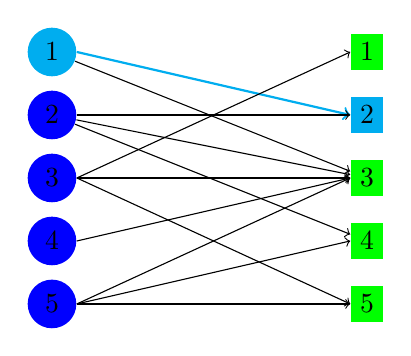
\begin{tikzpicture}
            % Boys
            \node[fill=cyan, circle] (p1) at (0,0) {1};
            \node[fill=blue, circle] (p2) at (0,-0.8) {2};
            \node[fill=blue, circle] (p3) at (0,-1.6) {3};
             \node[fill=blue, circle] (p4) at (0,-2.4) {4};
            \node[fill=blue, circle] (p5) at (0,-3.2) {5};
             
            
            
            % Girls
            \node[fill=green, rectangle] (f1) at (4,0) {1};
            \node[fill=cyan, rectangle] (f2) at (4,-0.8) {2};
            \node[fill=green, rectangle] (f3) at (4,-1.6) {3};
            \node[fill=green, rectangle] (f4) at (4,-2.4) {4};
            \node[fill=green, rectangle] (f5) at (4,-3.2) {5};
            
            % Potential Pairs
           \draw[cyan,thick,->] (p1.east) --  (f2.west);
            \draw[->] (p1) -- (f3);
            \draw[->] (p2) -- (f2);
            \draw[->] (p2) -- (f3);
            \draw[->] (p2) -- (f4);
             \draw[->] (p3.east) -- (f1.west);
              \draw[->] (p3.east) -- (f3.west);
               \draw[->] (p3.east) -- (f5.west);
                \draw[->] (p4.east) -- (f3.west);
                  \draw[->] (p5.east) -- (f3.west);
               \draw[->] (p5.east) -- (f5.west);
                \draw[->] (p5.east) -- (f4.west);
            
            
            

        \end{tikzpicture}
    \end{frame}
        \begin{frame}{Greedy Approach}
        
    Here,item 2 was already taken by person 1
    \vspace{2 pt}

        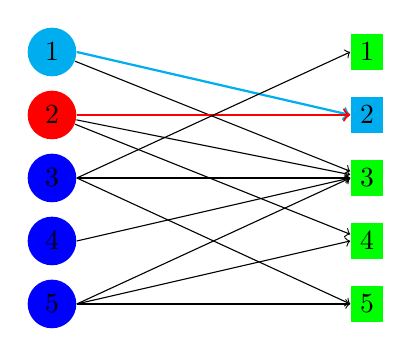
\begin{tikzpicture}
            % Boys
            \node[fill=cyan, circle] (p1) at (0,0) {1};
            \node[fill=red, circle] (p2) at (0,-0.8) {2};
            \node[fill=blue, circle] (p3) at (0,-1.6) {3};
             \node[fill=blue, circle] (p4) at (0,-2.4) {4};
            \node[fill=blue, circle] (p5) at (0,-3.2) {5};
             
            
            
            % Girls
            \node[fill=green, rectangle] (f1) at (4,0) {1};
            \node[fill=cyan, rectangle] (f2) at (4,-0.8) {2};
            \node[fill=green, rectangle] (f3) at (4,-1.6) {3};
            \node[fill=green, rectangle] (f4) at (4,-2.4) {4};
            \node[fill=green, rectangle] (f5) at (4,-3.2) {5};
            
            % Potential Pairs
           \draw[cyan,thick,->] (p1.east) --  (f2.west);
            \draw[->] (p1) -- (f3);
            \draw[red,thick,->] (p2) -- (f2);
            \draw[->] (p2) -- (f3);
            \draw[->] (p2) -- (f4);
             \draw[->] (p3.east) -- (f1.west);
              \draw[->] (p3.east) -- (f3.west);
               \draw[->] (p3.east) -- (f5.west);
                \draw[->] (p4.east) -- (f3.west);
                  \draw[->] (p5.east) -- (f3.west);
               \draw[->] (p5.east) -- (f5.west);
                \draw[->] (p5.east) -- (f4.west);
            
            
            

        \end{tikzpicture}
        
    \end{frame}
        \begin{frame}{Greedy Approach}
        
    

        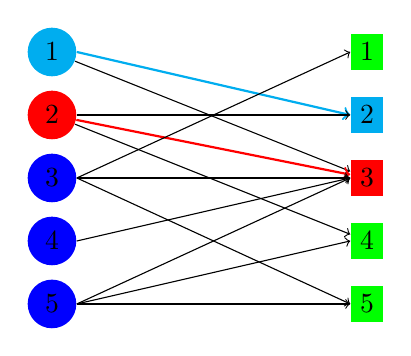
\begin{tikzpicture}
            % Boys
            \node[fill=cyan, circle] (p1) at (0,0) {1};
            \node[fill=red, circle] (p2) at (0,-0.8) {2};
            \node[fill=blue, circle] (p3) at (0,-1.6) {3};
             \node[fill=blue, circle] (p4) at (0,-2.4) {4};
            \node[fill=blue, circle] (p5) at (0,-3.2) {5};
             
            
            
            % Girls
            \node[fill=green, rectangle] (f1) at (4,0) {1};
            \node[fill=cyan, rectangle] (f2) at (4,-0.8) {2};
            \node[fill=red, rectangle] (f3) at (4,-1.6) {3};
            \node[fill=green, rectangle] (f4) at (4,-2.4) {4};
            \node[fill=green, rectangle] (f5) at (4,-3.2) {5};
            
            % Potential Pairs
           \draw[cyan,thick,->] (p1.east) --  (f2.west);
            \draw[->] (p1) -- (f3);
            \draw[->] (p2) -- (f2);
            \draw[red,thick,->] (p2) -- (f3);
            \draw[->] (p2) -- (f4);
             \draw[->] (p3.east) -- (f1.west);
              \draw[->] (p3.east) -- (f3.west);
               \draw[->] (p3.east) -- (f5.west);
                \draw[->] (p4.east) -- (f3.west);
                  \draw[->] (p5.east) -- (f3.west);
               \draw[->] (p5.east) -- (f5.west);
                \draw[->] (p5.east) -- (f4.west);
            
            
            

        \end{tikzpicture}
        
    \end{frame}
            \begin{frame}{Greedy Approach}
        
    Here,item 1 was luckily unoccupied 
    \vspace{2 pt}

        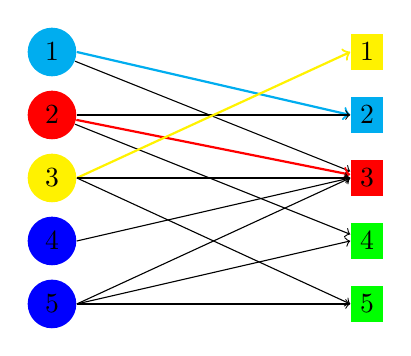
\begin{tikzpicture}
            % Boys
            \node[fill=cyan, circle] (p1) at (0,0) {1};
            \node[fill=red, circle] (p2) at (0,-0.8) {2};
            \node[fill=yellow, circle] (p3) at (0,-1.6) {3};
             \node[fill=blue, circle] (p4) at (0,-2.4) {4};
            \node[fill=blue, circle] (p5) at (0,-3.2) {5};
             
            
            
            % Girls
            \node[fill=yellow, rectangle] (f1) at (4,0) {1};
            \node[fill=cyan, rectangle] (f2) at (4,-0.8) {2};
            \node[fill=red, rectangle] (f3) at (4,-1.6) {3};
            \node[fill=green, rectangle] (f4) at (4,-2.4) {4};
            \node[fill=green, rectangle] (f5) at (4,-3.2) {5};
            
            % Potential Pairs
           \draw[cyan,thick,->] (p1.east) --  (f2.west);
            \draw[->] (p1) -- (f3);
            \draw[->] (p2) -- (f2);
            \draw[red,thick,->] (p2) -- (f3);
            \draw[->] (p2) -- (f4);
             \draw[yellow,thick,->] (p3.east) -- (f1.west);
              \draw[->] (p3.east) -- (f3.west);
               \draw[->] (p3.east) -- (f5.west);
                \draw[->] (p4.east) -- (f3.west);
                  \draw[->] (p5.east) -- (f3.west);
               \draw[->] (p5.east) -- (f5.west);
                \draw[->] (p5.east) -- (f4.west);
            
            
            

        \end{tikzpicture}
        
    \end{frame}
                \begin{frame}{Greedy Approach}
        
    Here,person 4 can not have anything and person 5 got a match luckily.
    \vspace{2 pt}

        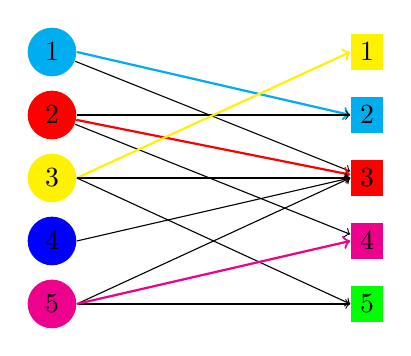
\begin{tikzpicture}
            % Boys
            \node[fill=cyan, circle] (p1) at (0,0) {1};
            \node[fill=red, circle] (p2) at (0,-0.8) {2};
            \node[fill=yellow, circle] (p3) at (0,-1.6) {3};
             \node[fill=blue, circle] (p4) at (0,-2.4) {4};
            \node[fill=magenta, circle] (p5) at (0,-3.2) {5};
             
            
            
            % Girls
            \node[fill=yellow, rectangle] (f1) at (4,0) {1};
            \node[fill=cyan, rectangle] (f2) at (4,-0.8) {2};
            \node[fill=red, rectangle] (f3) at (4,-1.6) {3};
            \node[fill=magenta, rectangle] (f4) at (4,-2.4) {4};
            \node[fill=green, rectangle] (f5) at (4,-3.2) {5};
            
            % Potential Pairs
           \draw[cyan,thick,->] (p1.east) --  (f2.west);
            \draw[->] (p1) -- (f3);
            \draw[->] (p2) -- (f2);
            \draw[red,thick,->] (p2) -- (f3);
            \draw[->] (p2) -- (f4);
             \draw[yellow,thick,->] (p3.east) -- (f1.west);
              \draw[->] (p3.east) -- (f3.west);
               \draw[->] (p3.east) -- (f5.west);
                \draw[->] (p4.east) -- (f3.west);
                  \draw[->] (p5.east) -- (f3.west);
               \draw[->] (p5.east) -- (f5.west);
                \draw[magenta,thick,->] (p5.east) -- (f4.west);
            
            
            

        \end{tikzpicture}

        We could only satisfy four guests.One guest is unhappy.
        
    \end{frame}
\section{Reducing to Network Flow}
\begin{frame}{Approach to solve }
    \begin{columns}[T]
        \begin{column}{0.4\textwidth}
            % Text column
            \begin{itemize}
                \item Given an instance of Bipartrite matching
                \item Reduce it to Max Flow Problem.
                \item 
Where the solution to the
network 
ow problem can
easily be used to find the
solution to the bipartite
matching.
            \end{itemize}
        \end{column}
        
        \begin{column}{0.5\textwidth}
            % Flowchart column
            \begin{figure}
                \centering
                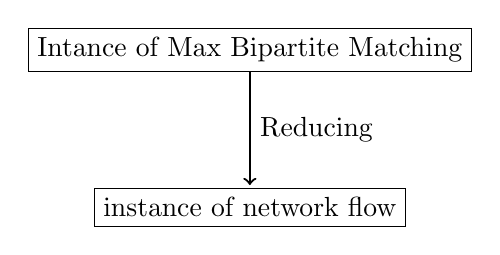
\begin{tikzpicture}[shorten >=1pt,node distance=2cm,auto]
                    % Nodes
                    \node[draw,rectangle] (A1) {Intance of Max Bipartite Matching};
                    \node[draw,rectangle] (B5) [below of=A1] {instance of network flow};
                
                    % Arrow
                    \draw[black,thick,->] (A1.south) -- node[midway, right] {Reducing} (B5.north);
                \end{tikzpicture}
            \end{figure}
        \end{column}
    \end{columns}
\end{frame}
\begin{frame}{Reducing to Network Flow Problem}
\textbf{Approach: }\\
    \begin{itemize}
        \item Make all the edges directed if not and add 0 flow and 1 capacity for all edges.Expressed as 0/1 in Flow/Capacity format
        \item add two new nodes: 
        \begin{enumerate}
            \item Source(S)
            \item Destination(t)
        \end{enumerate}
        \item 
        Add nodes from source to People with flow/capacity=0/1.
        \item 
        Add nodes from food items to destination with 0 flow and 1 capacity
        \item After applying network flow algorithm, flow>0 between the pairs indicates a matching.
        
    \end{itemize}
    
\end{frame}

\begin{frame}{Reduced to Network Flow}


        \begin{tikzpicture}
            \node[fill=yellow,rectangle](s) at (-3,-1.6) {S};
            \node[fill=brown,rectangle](t) at (7,-1.6) {t};

            \draw[->](s.east)--node[right,above,font=\small]{0/1} (p1.west);
            \draw[->](s.east)--node[midway,right,font=\small]{0/1} (p2.west);
            \draw[->](s.east)--node[midway,left,font=\small]{0/1} (p3.west);
            \draw[->](s.east)--node[midway,right,font=\small]{0/1} (p4.west);
            \draw[->](s.east)--node[midway,left,font=\small]{0/1} (p5.west);


            \draw[->](f1.east)--node[midway,above,font=\small]{0/1} (t.west);
            \draw[->](f2.east)--node[midway,left,font=\small]{0/1} (t.west);
            \draw[->](f3.east)--node[left,right,font=\small]{0/1} (t.west);
            \draw[->](f4.east)--node[left,right,font=\small]{0/1} (t.west);
            \draw[->](f5.east)--node[left,right,font=\small]{0/1} (t.west);


            
            \node[fill=blue, circle] (p1) at (0,0) {1};
            \node[fill=blue, circle] (p2) at (0,-0.8) {2};
            \node[fill=blue, circle] (p3) at (0,-1.6) {3};
             \node[fill=blue, circle] (p4) at (0,-2.4) {4};
            \node[fill=blue, circle] (p5) at (0,-3.2) {5};
             
            
            
            
            \node[fill=green, rectangle] (f1) at (4,0) {1};
            \node[fill=green, rectangle] (f2) at (4,-0.8) {2};
            \node[fill=green, rectangle] (f3) at (4,-1.6) {3};
            \node[fill=green, rectangle] (f4) at (4,-2.4) {4};
            \node[fill=green, rectangle] (f5) at (4,-3.2) {5};
            
            % Potential Pairs
            \draw[->] (p1.east)--node[midway,above,font=\small]{0/1}  (f2.west);
            \draw[->] (p1) -- node[near start,left,font=\small]{0/1}  (f3);
            \draw[->] (p2) -- node[near end,left,font=\small]{0/1}  (f2);
            \draw[->] (p2) -- node[midway,right,font=\small]{0/1}  (f3);
            \draw[->] (p2) -- node[near end,right,font=\small]{0/1} (f4);
             \draw[->] (p3.east) -- node[near end,right,font=\small]{0/1}  (f1.west);
              \draw[->] (p3.east) -- node[near end,right,font=\small]{0/1}  (f3.west);
               \draw[->] (p3.east) -- node[near end,right,font=\small]{0/1}  (f5.west);
                \draw[->] (p4.east) -- node[near start,above,font=\small]{0/1}  (f3.west);
                  \draw[->] (p5.east) -- node[near start,above,font=\small]{0/1} (f3.west);
               \draw[->] (p5.east) -- node[near end,below,font=\small]{0/1}  (f5.west);
                \draw[->] (p5.east) -- node[near end,above,font=\small]{0/1} (f4.west);
            
            
            

        \end{tikzpicture}
    
    
\end{frame}

\begin{frame}{Edmonds-Karp Algorithm to Solve Network Flow Problem}
        \begin{itemize}
        \item Initialize flow $f(u,v) = 0$ for all edges $(u,v)$ in the graph.
        \item Repeat the following steps until no augmenting paths can be found:
        \begin{itemize}
            \item Use BFS to find the shortest augmenting path from source to sink.
            \item If no augmenting path is found, terminate.
            \item Let $P$ be the augmenting path found by BFS.
            \item Let $cf(P)$ be the minimum residual capacity along path $P$.
            \item For each edge $(u,v)$ in $P$:
            \begin{itemize}
                \item Update flow $f(u,v) = f(u,v) + cf(P)$.
                \item Update flow $f(v,u) = f(v,u) - cf(P)$ for the reverse edge.
            \end{itemize}
        \end{itemize}
        \item The value of the maximum flow is the sum of flow values leaving the source.
    \end{itemize}

\end{frame}
\section{Solution}
\begin{frame}{Solution to Network Flow Problem}


        \begin{tikzpicture}
            \node[fill=yellow,rectangle](s) at (-3,-1.6) {S};
            \node[fill=brown,rectangle](t) at (7,-1.6) {t};

            \draw[brown,->](s.east)--node[right,above,font=\small]{1/1} (p1.west);
            \draw[->](s.east)--node[midway,right,font=\small]{0/1} (p2.west);
            \draw[->](s.east)--node[midway,left,font=\small]{0/1} (p3.west);
            \draw[->](s.east)--node[midway,right,font=\small]{0/1} (p4.west);
            \draw[->](s.east)--node[midway,left,font=\small]{0/1} (p5.west);


            \draw[->](f1.east)--node[midway,above,font=\small]{0/1} (t.west);
            \draw[brown,->](f2.east)--node[midway,left,font=\small]{1/1} (t.west);
            \draw[->](f3.east)--node[left,right,font=\small]{0/1} (t.west);
            \draw[->](f4.east)--node[left,right,font=\small]{0/1} (t.west);
            \draw[->](f5.east)--node[left,right,font=\small]{0/1} (t.west);


            
            \node[fill=blue, circle] (p1) at (0,0) {1};
            \node[fill=blue, circle] (p2) at (0,-0.8) {2};
            \node[fill=blue, circle] (p3) at (0,-1.6) {3};
             \node[fill=blue, circle] (p4) at (0,-2.4) {4};
            \node[fill=blue, circle] (p5) at (0,-3.2) {5};
             
            
            
            
            \node[fill=green, rectangle] (f1) at (4,0) {1};
            \node[fill=green, rectangle] (f2) at (4,-0.8) {2};
            \node[fill=green, rectangle] (f3) at (4,-1.6) {3};
            \node[fill=green, rectangle] (f4) at (4,-2.4) {4};
            \node[fill=green, rectangle] (f5) at (4,-3.2) {5};
            
            % Potential Pairs
            \draw[brown,->] (p1.east)--node[midway,above,font=\small]{1/1}  (f2.west);
            \draw[->] (p1) -- node[near start,left,font=\small]{0/1}  (f3);
            \draw[->] (p2) -- node[near end,left,font=\small]{0/1}  (f2);
            \draw[->] (p2) -- node[midway,right,font=\small]{0/1}  (f3);
            \draw[->] (p2) -- node[near end,right,font=\small]{0/1} (f4);
             \draw[->] (p3.east) -- node[near end,right,font=\small]{0/1}  (f1.west);
              \draw[->] (p3.east) -- node[near end,right,font=\small]{0/1}  (f3.west);
               \draw[->] (p3.east) -- node[near end,right,font=\small]{0/1}  (f5.west);
                \draw[->] (p4.east) -- node[near start,above,font=\small]{0/1}  (f3.west);
                  \draw[->] (p5.east) -- node[near start,above,font=\small]{0/1} (f3.west);
               \draw[->] (p5.east) -- node[near end,below,font=\small]{0/1}  (f5.west);
                \draw[->] (p5.east) -- node[near end,above,font=\small]{0/1} (f4.west);
            
            
            

        \end{tikzpicture}
    
    
\end{frame}

\begin{frame}{Solution to Network Flow Problem}


        \begin{tikzpicture}
            \node[fill=yellow,rectangle](s) at (-3,-1.6) {S};
            \node[fill=brown,rectangle](t) at (7,-1.6) {t};

            \draw[brown,->](s.east)--node[right,above,font=\small]{1/1} (p1.west);
            \draw[brown,->](s.east)--node[midway,right,font=\small]{1/1} (p2.west);
            \draw[->](s.east)--node[midway,left,font=\small]{0/1} (p3.west);
            \draw[->](s.east)--node[midway,right,font=\small]{0/1} (p4.west);
            \draw[->](s.east)--node[midway,left,font=\small]{0/1} (p5.west);


            \draw[->](f1.east)--node[midway,above,font=\small]{0/1} (t.west);
            \draw[brown,->](f2.east)--node[midway,left,font=\small]{1/1} (t.west);
            \draw[->](f3.east)--node[left,right,font=\small]{0/1} (t.west);
            \draw[brown,->](f4.east)--node[left,right,font=\small]{1/1} (t.west);
            \draw[->](f5.east)--node[left,right,font=\small]{0/1} (t.west);


            
            \node[fill=blue, circle] (p1) at (0,0) {1};
            \node[fill=blue, circle] (p2) at (0,-0.8) {2};
            \node[fill=blue, circle] (p3) at (0,-1.6) {3};
             \node[fill=blue, circle] (p4) at (0,-2.4) {4};
            \node[fill=blue, circle] (p5) at (0,-3.2) {5};
             
            
            
            
            \node[fill=green, rectangle] (f1) at (4,0) {1};
            \node[fill=green, rectangle] (f2) at (4,-0.8) {2};
            \node[fill=green, rectangle] (f3) at (4,-1.6) {3};
            \node[fill=green, rectangle] (f4) at (4,-2.4) {4};
            \node[fill=green, rectangle] (f5) at (4,-3.2) {5};
            
            % Potential Pairs
            \draw[brown,->] (p1.east)--node[midway,above,font=\small]{1/1}  (f2.west);
            \draw[->] (p1) -- node[near start,left,font=\small]{0/1}  (f3);
            \draw[->] (p2) -- node[near end,left,font=\small]{0/1}  (f2);
            \draw[->] (p2) -- node[midway,right,font=\small]{0/1}  (f3);
            \draw[brown,->] (p2) -- node[near end,right,font=\small]{1/1} (f4);
             \draw[->] (p3.east) -- node[near end,right,font=\small]{0/1}  (f1.west);
              \draw[->] (p3.east) -- node[near end,right,font=\small]{0/1}  (f3.west);
               \draw[->] (p3.east) -- node[near end,right,font=\small]{0/1}  (f5.west);
                \draw[->] (p4.east) -- node[near start,above,font=\small]{0/1}  (f3.west);
                  \draw[->] (p5.east) -- node[near start,above,font=\small]{0/1} (f3.west);
               \draw[->] (p5.east) -- node[near end,below,font=\small]{0/1}  (f5.west);
                \draw[->] (p5.east) -- node[near end,above,font=\small]{0/1} (f4.west);
            
            
            

        \end{tikzpicture}
    
    
\end{frame}

\begin{frame}{Solution to Network Flow Problem}


        \begin{tikzpicture}
            \node[fill=yellow,rectangle](s) at (-3,-1.6) {S};
            \node[fill=brown,rectangle](t) at (7,-1.6) {t};

            \draw[brown,->](s.east)--node[right,above,font=\small]{1/1} (p1.west);
            \draw[brown,->](s.east)--node[midway,right,font=\small]{1/1} (p2.west);
            \draw[brown,->](s.east)--node[midway,left,font=\small]{1/1} (p3.west);
            \draw[->](s.east)--node[midway,right,font=\small]{0/1} (p4.west);
            \draw[->](s.east)--node[midway,left,font=\small]{0/1} (p5.west);


            \draw[brown,->](f1.east)--node[midway,above,font=\small]{1/1} (t.west);
            \draw[brown,->](f2.east)--node[midway,left,font=\small]{1/1} (t.west);
            \draw[->](f3.east)--node[left,right,font=\small]{0/1} (t.west);
            \draw[brown,->](f4.east)--node[left,right,font=\small]{1/1} (t.west);
            \draw[->](f5.east)--node[left,right,font=\small]{0/1} (t.west);


            
            \node[fill=blue, circle] (p1) at (0,0) {1};
            \node[fill=blue, circle] (p2) at (0,-0.8) {2};
            \node[fill=blue, circle] (p3) at (0,-1.6) {3};
             \node[fill=blue, circle] (p4) at (0,-2.4) {4};
            \node[fill=blue, circle] (p5) at (0,-3.2) {5};
             
            
            
            
            \node[fill=green, rectangle] (f1) at (4,0) {1};
            \node[fill=green, rectangle] (f2) at (4,-0.8) {2};
            \node[fill=green, rectangle] (f3) at (4,-1.6) {3};
            \node[fill=green, rectangle] (f4) at (4,-2.4) {4};
            \node[fill=green, rectangle] (f5) at (4,-3.2) {5};
            
            % Potential Pairs
            \draw[brown,->] (p1.east)--node[midway,above,font=\small]{1/1}  (f2.west);
            \draw[->] (p1) -- node[near start,left,font=\small]{0/1}  (f3);
            \draw[->] (p2) -- node[near end,left,font=\small]{0/1}  (f2);
            \draw[->] (p2) -- node[midway,right,font=\small]{0/1}  (f3);
            \draw[brown,->] (p2) -- node[near end,right,font=\small]{1/1} (f4);
             \draw[brown,->] (p3.east) -- node[near end,right,font=\small]{1/1}  (f1.west);
              \draw[->] (p3.east) -- node[near end,right,font=\small]{0/1}  (f3.west);
               \draw[->] (p3.east) -- node[near end,right,font=\small]{0/1}  (f5.west);
                \draw[->] (p4.east) -- node[near start,above,font=\small]{0/1}  (f3.west);
                  \draw[->] (p5.east) -- node[near start,above,font=\small]{0/1} (f3.west);
               \draw[->] (p5.east) -- node[near end,below,font=\small]{0/1}  (f5.west);
                \draw[->] (p5.east) -- node[near end,above,font=\small]{0/1} (f4.west);
            
            
            

        \end{tikzpicture}
    
    
\end{frame}

\begin{frame}{Solution to Network Flow Problem}


        \begin{tikzpicture}
            \node[fill=yellow,rectangle](s) at (-3,-1.6) {S};
            \node[fill=brown,rectangle](t) at (7,-1.6) {t};

            \draw[brown,->](s.east)--node[right,above,font=\small]{1/1} (p1.west);
            \draw[brown,->](s.east)--node[midway,right,font=\small]{1/1} (p2.west);
            \draw[brown,->](s.east)--node[midway,left,font=\small]{1/1} (p3.west);
            \draw[brown,->](s.east)--node[midway,right,font=\small]{1/1} (p4.west);
            \draw[->](s.east)--node[midway,left,font=\small]{0/1} (p5.west);


            \draw[brown,->](f1.east)--node[midway,above,font=\small]{1/1} (t.west);
            \draw[brown,->](f2.east)--node[midway,left,font=\small]{1/1} (t.west);
            \draw[brown,->](f3.east)--node[left,right,font=\small]{1/1} (t.west);
            \draw[brown,->](f4.east)--node[left,right,font=\small]{1/1} (t.west);
            \draw[->](f5.east)--node[left,right,font=\small]{0/1} (t.west);


            
            \node[fill=blue, circle] (p1) at (0,0) {1};
            \node[fill=blue, circle] (p2) at (0,-0.8) {2};
            \node[fill=blue, circle] (p3) at (0,-1.6) {3};
             \node[fill=blue, circle] (p4) at (0,-2.4) {4};
            \node[fill=blue, circle] (p5) at (0,-3.2) {5};
             
            
            
            
            \node[fill=green, rectangle] (f1) at (4,0) {1};
            \node[fill=green, rectangle] (f2) at (4,-0.8) {2};
            \node[fill=green, rectangle] (f3) at (4,-1.6) {3};
            \node[fill=green, rectangle] (f4) at (4,-2.4) {4};
            \node[fill=green, rectangle] (f5) at (4,-3.2) {5};
            
            % Potential Pairs
            \draw[brown,->] (p1.east)--node[midway,above,font=\small]{1/1}  (f2.west);
            \draw[->] (p1) -- node[near start,left,font=\small]{0/1}  (f3);
            \draw[->] (p2) -- node[near end,left,font=\small]{0/1}  (f2);
            \draw[->] (p2) -- node[midway,right,font=\small]{0/1}  (f3);
            \draw[brown,->] (p2) -- node[near end,right,font=\small]{1/1} (f4);
             \draw[brown,->] (p3.east) -- node[near end,right,font=\small]{1/1}  (f1.west);
              \draw[->] (p3.east) -- node[near end,right,font=\small]{0/1}  (f3.west);
               \draw[->] (p3.east) -- node[near end,right,font=\small]{0/1}  (f5.west);
                \draw[brown,->] (p4.east) -- node[near start,above,font=\small]{1/1}  (f3.west);
                  \draw[->] (p5.east) -- node[near start,above,font=\small]{0/1} (f3.west);
               \draw[->] (p5.east) -- node[near end,below,font=\small]{0/1}  (f5.west);
                \draw[->] (p5.east) -- node[near end,above,font=\small]{0/1} (f4.west);
            
            
            

        \end{tikzpicture}
    
    
\end{frame}

\begin{frame}{Solution to Network Flow Problem}


        \begin{tikzpicture}
            \node[fill=yellow,rectangle](s) at (-3,-1.6) {S};
            \node[fill=brown,rectangle](t) at (7,-1.6) {t};

            \draw[brown,->](s.east)--node[right,above,font=\small]{1/1} (p1.west);
            \draw[brown,->](s.east)--node[midway,right,font=\small]{1/1} (p2.west);
            \draw[brown,->](s.east)--node[midway,left,font=\small]{1/1} (p3.west);
            \draw[brown,->](s.east)--node[midway,right,font=\small]{1/1} (p4.west);
            \draw[brown,->](s.east)--node[midway,left,font=\small]{1/1} (p5.west);


            \draw[brown,->](f1.east)--node[midway,above,font=\small]{1/1} (t.west);
            \draw[brown,->](f2.east)--node[midway,left,font=\small]{1/1} (t.west);
            \draw[brown,->](f3.east)--node[left,right,font=\small]{1/1} (t.west);
            \draw[brown,->](f4.east)--node[left,right,font=\small]{1/1} (t.west);
            \draw[brown,->](f5.east)--node[left,right,font=\small]{1/1} (t.west);


            
            \node[fill=blue, circle] (p1) at (0,0) {1};
            \node[fill=blue, circle] (p2) at (0,-0.8) {2};
            \node[fill=blue, circle] (p3) at (0,-1.6) {3};
             \node[fill=blue, circle] (p4) at (0,-2.4) {4};
            \node[fill=blue, circle] (p5) at (0,-3.2) {5};
             
            
            
            
            \node[fill=green, rectangle] (f1) at (4,0) {1};
            \node[fill=green, rectangle] (f2) at (4,-0.8) {2};
            \node[fill=green, rectangle] (f3) at (4,-1.6) {3};
            \node[fill=green, rectangle] (f4) at (4,-2.4) {4};
            \node[fill=green, rectangle] (f5) at (4,-3.2) {5};
            
            % Potential Pairs
            \draw[brown,->] (p1.east)--node[midway,above,font=\small]{1/1}  (f2.west);
            \draw[->] (p1) -- node[near start,left,font=\small]{0/1}  (f3);
            \draw[->] (p2) -- node[near end,left,font=\small]{0/1}  (f2);
            \draw[->] (p2) -- node[midway,right,font=\small]{0/1}  (f3);
            \draw[brown,->] (p2) -- node[near end,right,font=\small]{1/1} (f4);
             \draw[brown,->] (p3.east) -- node[near end,right,font=\small]{1/1}  (f1.west);
              \draw[->] (p3.east) -- node[near end,right,font=\small]{0/1}  (f3.west);
               \draw[->] (p3.east) -- node[near end,right,font=\small]{0/1}  (f5.west);
                \draw[brown,->] (p4.east) -- node[near start,above,font=\small]{1/1}  (f3.west);
                  \draw[->] (p5.east) -- node[near start,above,font=\small]{0/1} (f3.west);
               \draw[brown,->] (p5.east) -- node[near end,below,font=\small]{1/1}  (f5.west);
                \draw[->] (p5.east) -- node[near end,above,font=\small]{0/1} (f4.west);
            
            
            

        \end{tikzpicture}

    
    
\end{frame}
\begin{frame}{Analyzing the solution}
            Here,we can not augment the paths anymore.We have already found the max flow of the network.The max flow=5.Hence,Number of matching=5.
        
        \textbf{Pairs are} : 
        \begin{enumerate}
            \item Person 1,Item 2
            \item Person 2,Item 4
            \item Person 3,Item 1
            \item Person 4,Item 3
            \item Person 5,Item 5
        \end{enumerate}
        Using greedy approach,we found 4 pairs which was not maximum.
\end{frame}
\section{Extension}
\begin{frame}{Extension of Maximum Bipartrite matching}
    \begin{block}{Allowing multiple items for a person}
    What if a person is allowed to take multiple items?
\end{block}
    \begin{block}{Solution}
        The capacity of edge connected the source and a person would be equal to the number of items that person is allowed to take.Then Network flow algorithm should be applied as usual.
    \end{block}
\end{frame}

\begin{frame}{Extension of Maximum Bipartrite matching}
For example if Person 2 is allowed to take 3 items and person 5 is allowed to take 2 items:

        \begin{tikzpicture}
            \node[fill=yellow,rectangle](s) at (-3,-1.6) {S};
            \node[fill=brown,rectangle](t) at (7,-1.6) {t};

            \draw[->](s.east)--node[right,above,font=\small]{0/1} (p1.west);
            \draw[->](s.east)--node[midway,right,font=\small]{0/\textcolor{red}{3}} (p2.west);
            \draw[->](s.east)--node[midway,left,font=\small]{0/1} (p3.west);
            \draw[->](s.east)--node[midway,right,font=\small]{0/1} (p4.west);
            \draw[->](s.east)--node[midway,left,font=\small]{0/\textcolor{red}{2}} (p5.west);


            \draw[->](f1.east)--node[midway,above,font=\small]{0/1} (t.west);
            \draw[->](f2.east)--node[midway,left,font=\small]{0/1} (t.west);
            \draw[->](f3.east)--node[left,right,font=\small]{0/1} (t.west);
            \draw[->](f4.east)--node[left,right,font=\small]{0/1} (t.west);
            \draw[->](f5.east)--node[left,right,font=\small]{0/1} (t.west);


            
            \node[fill=blue, circle] (p1) at (0,0) {1};
            \node[fill=blue, circle] (p2) at (0,-0.8) {2};
            \node[fill=blue, circle] (p3) at (0,-1.6) {3};
             \node[fill=blue, circle] (p4) at (0,-2.4) {4};
            \node[fill=blue, circle] (p5) at (0,-3.2) {5};
             
            
            
            
            \node[fill=green, rectangle] (f1) at (4,0) {1};
            \node[fill=green, rectangle] (f2) at (4,-0.8) {2};
            \node[fill=green, rectangle] (f3) at (4,-1.6) {3};
            \node[fill=green, rectangle] (f4) at (4,-2.4) {4};
            \node[fill=green, rectangle] (f5) at (4,-3.2) {5};
            
            % Potential Pairs
            \draw[->] (p1.east)--node[midway,above,font=\small]{0/1}  (f2.west);
            \draw[->] (p1) -- node[near start,left,font=\small]{0/1}  (f3);
            \draw[->] (p2) -- node[near end,left,font=\small]{0/1}  (f2);
            \draw[->] (p2) -- node[midway,right,font=\small]{0/1}  (f3);
            \draw[->] (p2) -- node[near end,right,font=\small]{0/1} (f4);
             \draw[->] (p3.east) -- node[near end,right,font=\small]{0/1}  (f1.west);
              \draw[->] (p3.east) -- node[near end,right,font=\small]{0/1}  (f3.west);
               \draw[->] (p3.east) -- node[near end,right,font=\small]{0/1}  (f5.west);
                \draw[->] (p4.east) -- node[near start,above,font=\small]{0/1}  (f3.west);
                  \draw[->] (p5.east) -- node[near start,above,font=\small]{0/1} (f3.west);
               \draw[->] (p5.east) -- node[near end,below,font=\small]{0/1}  (f5.west);
                \draw[->] (p5.east) -- node[near end,above,font=\small]{0/1} (f4.west);
            
            
            

        \end{tikzpicture}
    
    
\end{frame}
\begin{frame}{Extension of Maximum Bipartrite matching}
    \begin{block}{Multiple copies of item available }
    What if an item has multiple instances?
\end{block}
    \begin{block}{Solution}
        The capacity of edge connected the  item and Destination would be equal to the number of copies of the item . Then Network flow algorithm should be applied as usual.
    \end{block}
\end{frame}

\begin{frame}{Extension of Maximum Bipartrite matching}
For example if item 1 has 3 copies and item 5 has 4 copies:

        \begin{tikzpicture}
            \node[fill=yellow,rectangle](s) at (-3,-1.6) {S};
            \node[fill=brown,rectangle](t) at (7,-1.6) {t};

            \draw[->](s.east)--node[right,above,font=\small]{0/1} (p1.west);
            \draw[->](s.east)--node[midway,right,font=\small]{0/\textcolor{red}{3}} (p2.west);
            \draw[->](s.east)--node[midway,left,font=\small]{0/1} (p3.west);
            \draw[->](s.east)--node[midway,right,font=\small]{0/1} (p4.west);
            \draw[->](s.east)--node[midway,left,font=\small]{0/\textcolor{red}{2}} (p5.west);


            \draw[->](f1.east)--node[midway,above,font=\small]{0/\textcolor{red}{3}} (t.west);
            \draw[->](f2.east)--node[midway,left,font=\small]{0/1} (t.west);
            \draw[->](f3.east)--node[left,right,font=\small]{0/1} (t.west);
            \draw[->](f4.east)--node[left,right,font=\small]{0/1} (t.west);
            \draw[->](f5.east)--node[left,right,font=\small]{0/\textcolor{red}{4}} (t.west);


            
            \node[fill=blue, circle] (p1) at (0,0) {1};
            \node[fill=blue, circle] (p2) at (0,-0.8) {2};
            \node[fill=blue, circle] (p3) at (0,-1.6) {3};
             \node[fill=blue, circle] (p4) at (0,-2.4) {4};
            \node[fill=blue, circle] (p5) at (0,-3.2) {5};
             
            
            
            
            \node[fill=green, rectangle] (f1) at (4,0) {1};
            \node[fill=green, rectangle] (f2) at (4,-0.8) {2};
            \node[fill=green, rectangle] (f3) at (4,-1.6) {3};
            \node[fill=green, rectangle] (f4) at (4,-2.4) {4};
            \node[fill=green, rectangle] (f5) at (4,-3.2) {5};
            
            % Potential Pairs
            \draw[->] (p1.east)--node[midway,above,font=\small]{0/1}  (f2.west);
            \draw[->] (p1) -- node[near start,left,font=\small]{0/1}  (f3);
            \draw[->] (p2) -- node[near end,left,font=\small]{0/1}  (f2);
            \draw[->] (p2) -- node[midway,right,font=\small]{0/1}  (f3);
            \draw[->] (p2) -- node[near end,right,font=\small]{0/1} (f4);
             \draw[->] (p3.east) -- node[near end,right,font=\small]{0/1}  (f1.west);
              \draw[->] (p3.east) -- node[near end,right,font=\small]{0/1}  (f3.west);
               \draw[->] (p3.east) -- node[near end,right,font=\small]{0/1}  (f5.west);
                \draw[->] (p4.east) -- node[near start,above,font=\small]{0/1}  (f3.west);
                  \draw[->] (p5.east) -- node[near start,above,font=\small]{0/1} (f3.west);
               \draw[->] (p5.east) -- node[near end,below,font=\small]{0/1}  (f5.west);
                \draw[->] (p5.east) -- node[near end,above,font=\small]{0/1} (f4.west);
            
            
            

        \end{tikzpicture}
    
    
\end{frame}

\begin{frame}{Extension of Maximum Bipartrite matching}
    \begin{block}{Taking same item multiple times? }
    What if an item can be taken multiple times by a person?
\end{block}
    \begin{block}{Solution}
        The capacity of edge connected between the  person and the item would be equal to the number of times the item can be taken by that person. Then Network flow algorithm should be applied as usual.
    \end{block}
\end{frame}

\begin{frame}{Extension of Maximum Bipartrite matching}
For example if Person1 can take Item 2 upto 5 times:

        \begin{tikzpicture}
            \node[fill=yellow,rectangle](s) at (-3,-1.6) {S};
            \node[fill=brown,rectangle](t) at (7,-1.6) {t};

            \draw[->](s.east)--node[right,above,font=\small]{0/1} (p1.west);
            \draw[->](s.east)--node[midway,right,font=\small]{0/\textcolor{red}{3}} (p2.west);
            \draw[->](s.east)--node[midway,left,font=\small]{0/1} (p3.west);
            \draw[->](s.east)--node[midway,right,font=\small]{0/1} (p4.west);
            \draw[->](s.east)--node[midway,left,font=\small]{0/\textcolor{red}{2}} (p5.west);


            \draw[->](f1.east)--node[midway,above,font=\small]{0/\textcolor{red}{3}} (t.west);
            \draw[->](f2.east)--node[midway,left,font=\small]{0/1} (t.west);
            \draw[->](f3.east)--node[left,right,font=\small]{0/1} (t.west);
            \draw[->](f4.east)--node[left,right,font=\small]{0/1} (t.west);
            \draw[->](f5.east)--node[left,right,font=\small]{0/\textcolor{red}{4}} (t.west);


            
            \node[fill=blue, circle] (p1) at (0,0) {1};
            \node[fill=blue, circle] (p2) at (0,-0.8) {2};
            \node[fill=blue, circle] (p3) at (0,-1.6) {3};
             \node[fill=blue, circle] (p4) at (0,-2.4) {4};
            \node[fill=blue, circle] (p5) at (0,-3.2) {5};
             
            
            
            
            \node[fill=green, rectangle] (f1) at (4,0) {1};
            \node[fill=green, rectangle] (f2) at (4,-0.8) {2};
            \node[fill=green, rectangle] (f3) at (4,-1.6) {3};
            \node[fill=green, rectangle] (f4) at (4,-2.4) {4};
            \node[fill=green, rectangle] (f5) at (4,-3.2) {5};
            
            % Potential Pairs
            \draw[->] (p1.east)--node[midway,above,font=\small]{0/\textcolor{red}{5}}  (f2.west);
            \draw[->] (p1) -- node[near start,left,font=\small]{0/1}  (f3);
            \draw[->] (p2) -- node[near end,left,font=\small]{0/1}  (f2);
            \draw[->] (p2) -- node[midway,right,font=\small]{0/1}  (f3);
            \draw[->] (p2) -- node[near end,right,font=\small]{0/1} (f4);
             \draw[->] (p3.east) -- node[near end,right,font=\small]{0/1}  (f1.west);
              \draw[->] (p3.east) -- node[near end,right,font=\small]{0/1}  (f3.west);
               \draw[->] (p3.east) -- node[near end,right,font=\small]{0/1}  (f5.west);
                \draw[->] (p4.east) -- node[near start,above,font=\small]{0/1}  (f3.west);
                  \draw[->] (p5.east) -- node[near start,above,font=\small]{0/1} (f3.west);
               \draw[->] (p5.east) -- node[near end,below,font=\small]{0/1}  (f5.west);
                \draw[->] (p5.east) -- node[near end,above,font=\small]{0/1} (f4.west);

        \end{tikzpicture}
    
    
\end{frame}

\section{References}

\begin{frame}{References}
\bibliographystyle{amsalpha}
\bibliography{ref}
\end{frame}

\end{document}